%
% Interconnecting & Interfacing Quantum Networks
%

\section{Interconnecting \& interfacing quantum networks} \label{sec:inter} \index{Interfacing quantum networks}

\dropcap{A}{ny} global-scale network will inevitably comprise participants choosing to go about things their own way. The physical architecture and medium may vary from one subnetwork to the next, as may the QTCP policies they adopt. The key then is to construct efficient \textit{interconnects} between different levels of the network hierarchy, each of which may subscribe to their own QTCP policies and cross between different physical mediums. Note that the QTCP protocol presented here does not enforce any particular networking policies, but rather provides a high-level framework that can be customised essentially arbitrarily.

For example, the cost metrics and attributes employed at the intercontinental level would most certainly be very different to those in a small LAN. A small LAN might be running applications whereby they can easily reproduce packets and thereby tolerate packet loss. But for a warehouse-scale commercial quantum computing enterprise, responsible for performing one stage of a distributed quantum computation, the loss of a single packet could be extremely costly, requiring the entire computation to be performed completely from scratch due to no-cloning\index{No-cloning theorem} and no-measurement limitations, something that may not come cheaply.

Such interconnects will typically comprise a combination of:
\begin{itemize}
\item Packet switching\index{Packet!Switching}: such that packets can be arbitrarily switched between the different levels of the network hierarchy.
\item Physical interface: interconnect may be switching between different media. Such physical interfaces have costs associated with them. For example, coupling between free-space and fibre is typically very lossy. Sec.~\ref{sec:opt_inter} discusses optical interfacing with matter qubits, and Sec.~\ref{sec:hybrid} discusses hybrid architectures, where optics mediates entanglement generation between matter qubits.
\item Quantum memory\index{Quantum memory}: such that data can be buffered while it awaits its turn at being switched between networks, as different networks may have different loads and operate at different clock-rates. This is discussed in Sec.~\ref{sec:memory}.
\item Packet format conversion\index{Packet!Format conversion}: different levels of the network hierarchy may be employing entirely different cost metrics, attributes, and cost functions, requiring packet headers to be reformatted upon switching between networks.
\end{itemize}

The packet switching and quantum memory are implemented as quantum processes at nodes, using the usual quantum process formalism. The physical interface between different mediums, if there is one, could be very diverse, encompassing many types of physical systems, but can always be characterised using the quantum process formalism. Packet headers, which contain all formatting, cost, and routing information are represented entirely classically and communicated entirely by the classical network. Thus, this operation also takes place at nodes, but no quantum processes are taking place.

%
% Optical Interfacing
%

\subsection{Optical interfacing} \label{sec:opt_inter} \index{Optical!Interfacing}

\comment{More details and techniques here}

Unless the entire pipeline of quantum operations through the course of a protocol is all-optical, there will be a need to exchange information between physical systems, for example via light-matter interactions \cite{bib:Cohen-Tannoudji92}. We will now discuss optical interfacing with some of the significant types of matter systems, such that their intercommunication can be optically mediated over the network.

%
% Two-Level Systems
%

\subsubsection{Two-level systems} \index{Two-level systems}

The archetypal interface is that between a photonic qubit in the \mbox{$\{\ket{0},\ket{1}\}$} photon-number basis, and a two-level matter qubit\index{Matter qubits} in the $\ket{g}$ (ground) and $\ket{e}$ (excited) state basis. The logical qubit is defined as,
\begin{align}
	\ket{0}_L &\equiv \ket{g}, \nonumber \\
	\ket{1}_L &\equiv \ket{e}.
\end{align}.
Examples include atoms in cavities\index{Atoms in cavities}, NV centres\index{Nitrogen-vacancy (NV) centres}, and engineered quantum dots\index{Quantum dots}.

In the case of a photon interacting with a two-level matter qubit, the interface can be expressed via the Jaynes-Cummings\index{Jaynes-Cummings Hamiltonian} interaction Hamiltonian of the form,
\begin{align} \label{eq:two_level_hamil}
\hat{H}_\mathrm{int} = \hbar \chi (\hat{a}\,\hat\sigma^+ + \hat{a}^\dag\hat\sigma^-),
\end{align}
where $\hat{a}$ ($\hat{a}^\dag$) is the photonic annihilation (creation) operator, $\hat\sigma^\pm$ are the Pauli spin-flip operators, and $\chi$ is the interaction strength\index{Interaction strength}. The interpretation of this Hamiltonian is very clear upon inspection -- the annihilation (creation) of a photon is associated with the excitation (relaxation) of the two-level matter system, thereby directly coherently exchanging quantum information between the two systems, as shown in Fig.~\ref{fig:opt_int}.

\begin{figure}[!htbp]
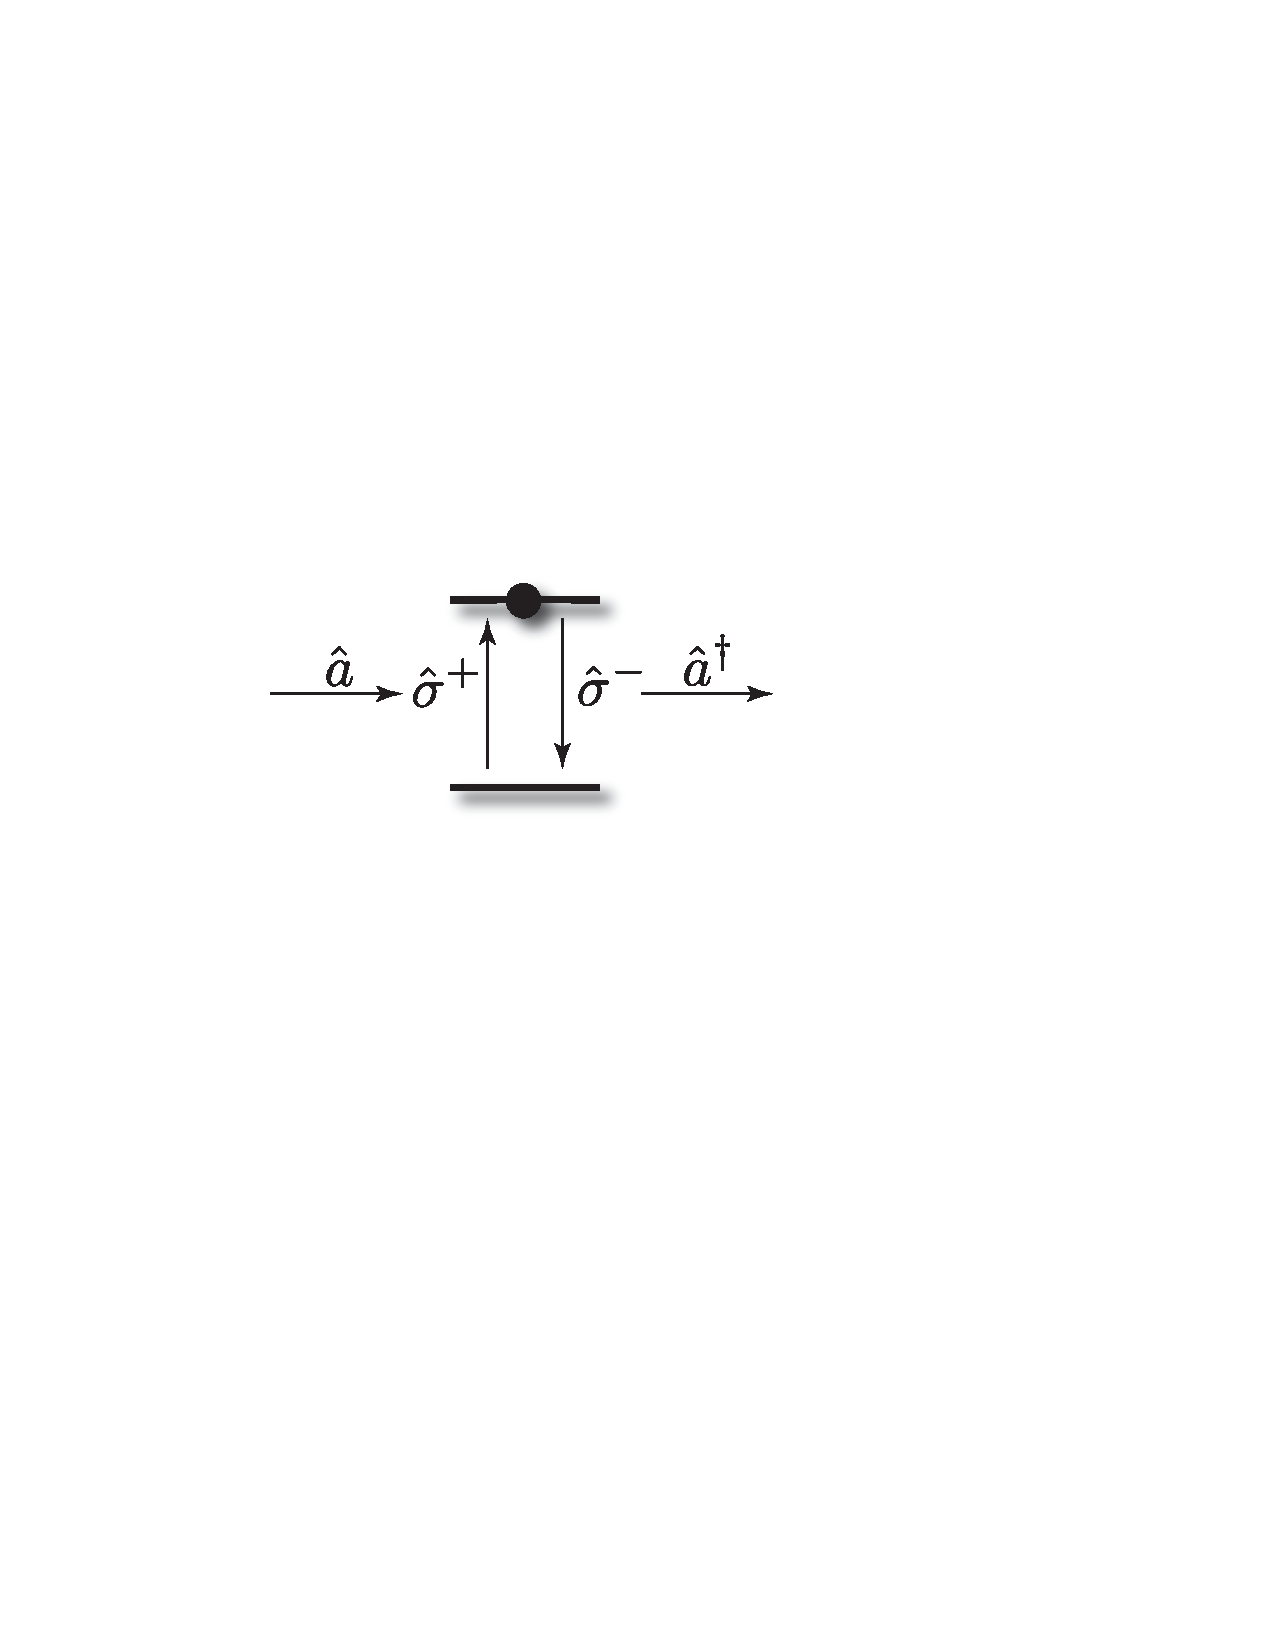
\includegraphics[clip=true, width=0.3\textwidth]{opt_inter}
\captionspacefig \caption{Light-matter interfacing between a single-photon state ($\hat{a}$, $\hat{a}^\dag$) and a two-level matter qubit ($\ket{g}$, $\ket{e}$). The absorption (emission) of a photon is associated with the excitation (relaxation) of the matter qubit ($\hat\sigma^\pm$).} \label{fig:opt_int}
\end{figure}

%
% Lambda-Configuration Systems
%

\subsubsection{$\lambda$-configuration systems} \index{$\lambda$-configuration systems}

Alternately, one can easily optically interface with a $\lambda$-configuration system, as shown in Fig.~\ref{fig:lambda_atom}. Here there are two degenerate ground states representing the logical qubit basis states (\mbox{$\ket{0}_L\equiv\ket{\!\uparrow}$}, \mbox{$\ket{1}_L\equiv\ket{\!\downarrow}$}), one of which may undergo a transition to an excited state, $\ket{e}$. By pumping the system to the excited state and waiting for a coherent relaxation, the emitted photon may be used to couple the qubit state of the $\lambda$-configuration to an optical mode, mapping the qubit value of the matter qubit to a photon-number representation.

\begin{figure}[!htbp]
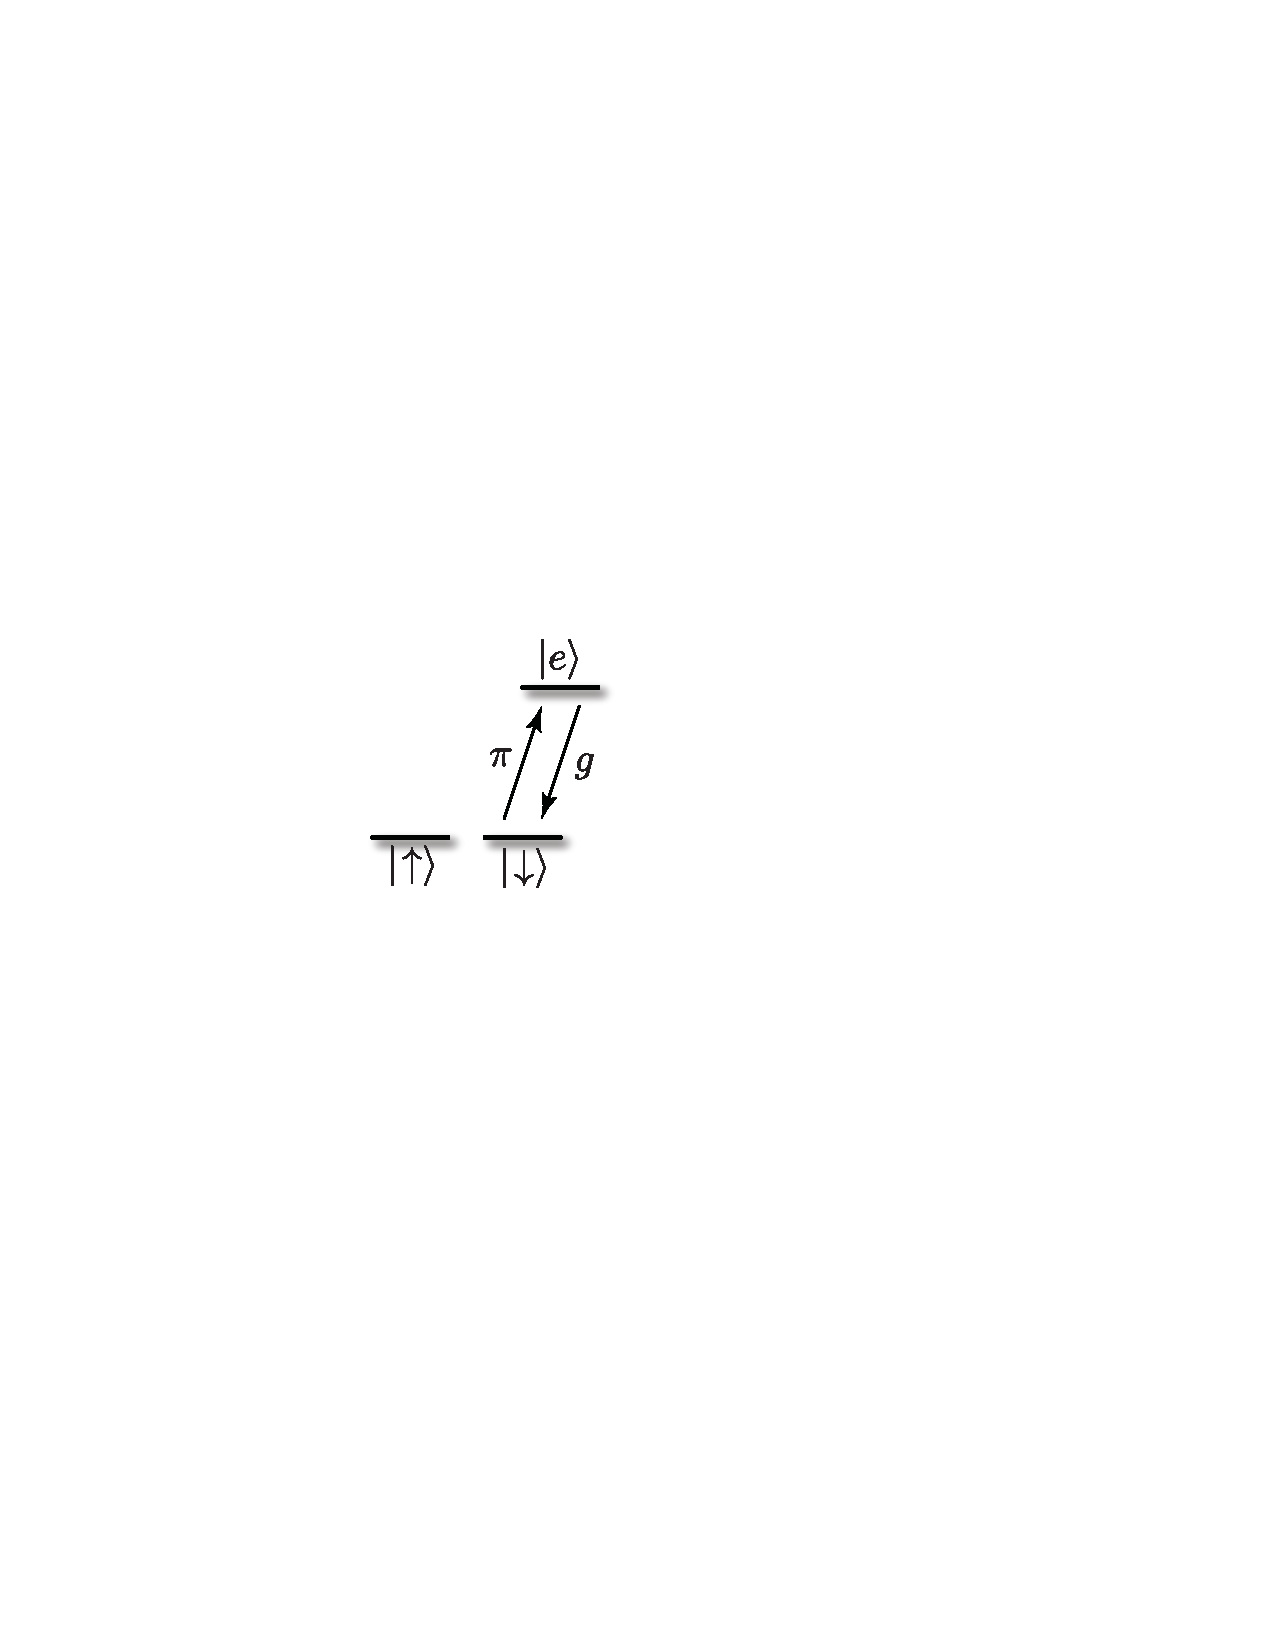
\includegraphics[clip=true, width=0.225\textwidth]{lambda_atom}
\captionspacefig \caption{Light-matter interfacing between an optical mode and a $\lambda$-configuration system. The two degenerate ground states represent the logical qubit (\mbox{$\ket{0}_L\equiv\ket{\!\uparrow}$}, \mbox{$\ket{1}_L\equiv\ket{\!\downarrow}$}), only one of which may undergo transition to the excited state $\ket{e}$. Upon pumping the \mbox{$\ket{\!\downarrow}\to\ket{e}$} transition with a $\pi$-pulse, a relaxation back to the ground state maps the logical qubit value to photon-number.} \label{fig:lambda_atom}
\end{figure}

%
% Atomic Ensembles
%

\subsubsection{Atomic ensembles} \label{sec:atomic_ens} \index{Atomic ensembles}

In addition to single atoms with well-defined electronic structure, atomic ensembles \cite{DLCZ, bib:Chou05} can be used, whereby the absorption of a photon creates a \textit{collective excitation}\index{Collective excitations} -- a superposition of a single excitation across all the atoms in the ensemble. Specifically, excitations are represented using collective excitation operators,
\begin{align}\index{Collective excitations!Operator}
\hat{S}^\dag = \frac{1}{\sqrt{N}}\sum_{i=1}^N \hat{S}_i^\dag,
\end{align}
where,
\begin{align}
\hat{S}_i^\dag=\ket{e}_i\bra{g}_i,
\end{align}
is the excitation operator for the $i$th atom in the ensemble, $\ket{g}_i$ and $\ket{e}_i$ are the ground and excited states for the $i$th particle, and there are $N$ atoms. The state of a single collective excitation is then given by,
\begin{align}
\ket{\psi_\mathrm{collective}} = \hat{S}^\dag \ket{g}^{\otimes N}.	
\end{align}

Atomic ensembles are essentially well-engineered clouds of atomic gasses, trapped in a glass container, coupled to an optical mode. Atomic ensembles have been demonstrated with extremely long coherence lifetimes ($T_2$-times on the order of milliseconds\index{T$_2$-time}), operating at room temperatures (a very attractive feature on its own). They exhibit \textit{collective enhancement}\index{Collective enhancement} in their coupling to the optical mode -- the optical coupling strength is amplified by a factor quadratic in $N$ compared to single-atom optical coupling, mitigating the need for a cavity.

The collective excitations exhibit the same general mathematical structure as single-atom excitations -- the absorption (emission) of a single photon is associated with a single collective excitation (relaxation), albeit with the favourable collective enhancement in the coupling strength.

To couple with a polarisation-encoded photonic qubit, a PBS can be employed to spatially separate the horizontal and vertical modes, each of which couples to a separate atomic ensemble, which jointly represent the logical qubit, as shown in Fig.~\ref{fig:atomic_ensemble_qubit}.

\begin{figure}[!htbp]
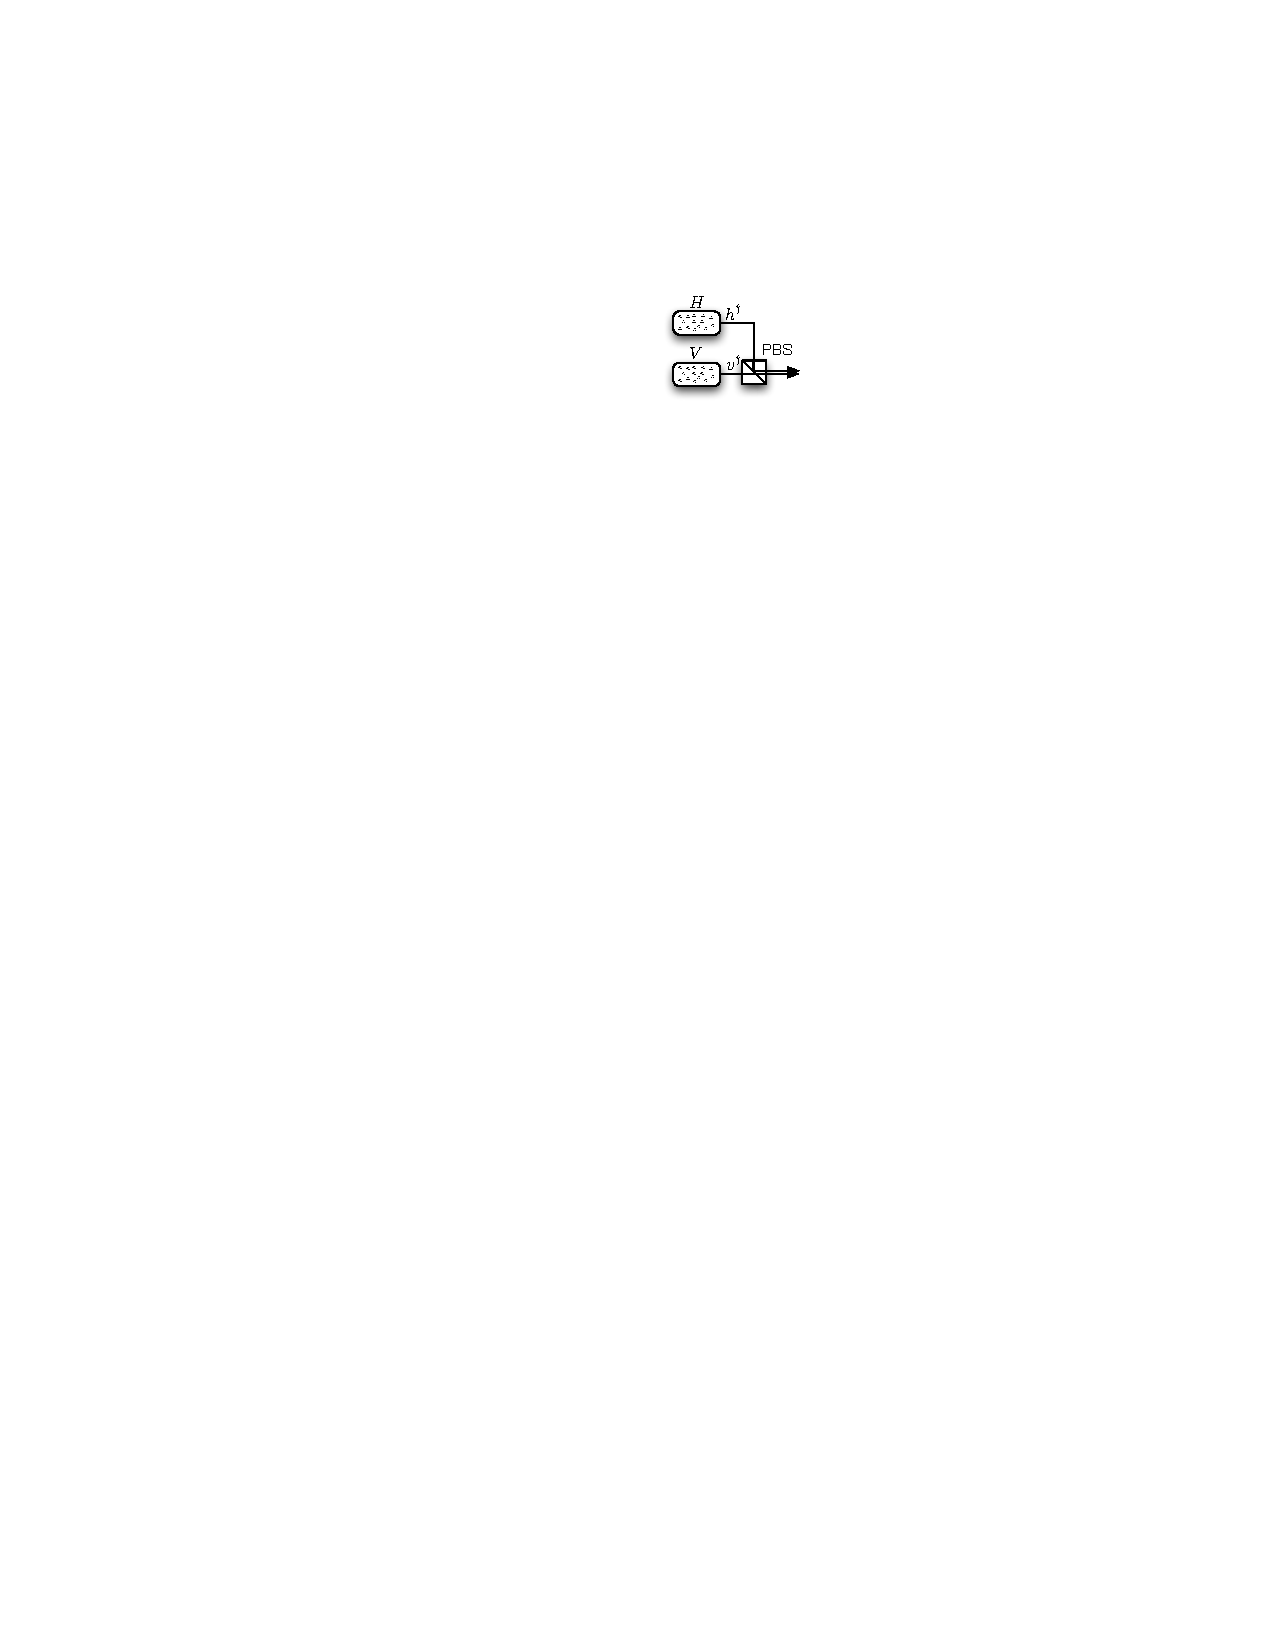
\includegraphics[clip=true, width=0.225\textwidth]{atomic_ensemble_qubit}
\captionspacefig \caption{Coupling a polarisation-encoded photonic qubit to a pair of atomic ensembles, each of which corresponds to one of the qubit's logical basis states ($\ket{0}$ or $\ket{1}$). The horizontal and vertical components of the photonic qubit are spatially separated using a PBS, which subsequently independently interface with distinct atomic ensembles via collective excitation.} \label{fig:atomic_ensemble_qubit}
\end{figure}

Atomic ensembles have been proposed as quantum memories, given their long coherence lifetimes. Additionally, a protocol for universal cluster state quantum computation (Sec.~\ref{sec:CSQC}) based upon atomic ensemble qubits has been described \cite{bib:RohdeAtEns10}.

Essentially, the long coherence lifetimes of collective excitations owes to the fact that the excitation is effectively encoded as a W-state (Sec.~\ref{sec:W_state_prep})\index{W-states}, an equal superposition of a single excitation across many ($N$) atoms, of the form,
\begin{align}
\ket{\psi_W^{(N)}} = \frac{1}{\sqrt{N}}(&\ket{e,g,g,\dots}\nonumber \\
+&\ket{g,e,g,\dots}\nonumber \\
+&\ket{g,g,e,\dots}\nonumber \\
+&\dots\nonumber \\
+&\ket{g,g,\dots,e}).
\end{align}
W-states are favourable from a decoherence perspective as tracing out a single particle has minimal impact on the coherence of the residual state, which preserves most entanglement, with this robustness growing with the number of particles. This is in stark contrast to GHZ states, which completely decohere under the loss of just a single particle.

Specifically, if $\ket{\psi_W^{(N)}}$ is the $N$-particle W-state (collective excitation), tracing out a single particle yields,
\begin{align}
\hat\rho_\mathrm{tr} &= \mathrm{tr}_1(\ket{\psi_W^{(N)}}\bra{\psi_W^{(N)}}) \\
&= \left(1-\frac{1}{N}\right)\ket{\psi_W^{(N-1)}}\bra{\psi_W^{(N-1)}} + \frac{1}{N}(\ket{g}\bra{g})^{\otimes (N-1)}, \nonumber
\end{align}
which for \mbox{$N\gg 1$} approaches the pure state $\ket{\psi_W^{(N-1)}}$, i.e a W-state with one fewer particles.

%
% Microwave Qubits
%

\subsubsection{Microwave qubits}

\comment{To do. Jon Dowling.}